\section{Оборудование}
\begin{figure}[ht!]
    \centering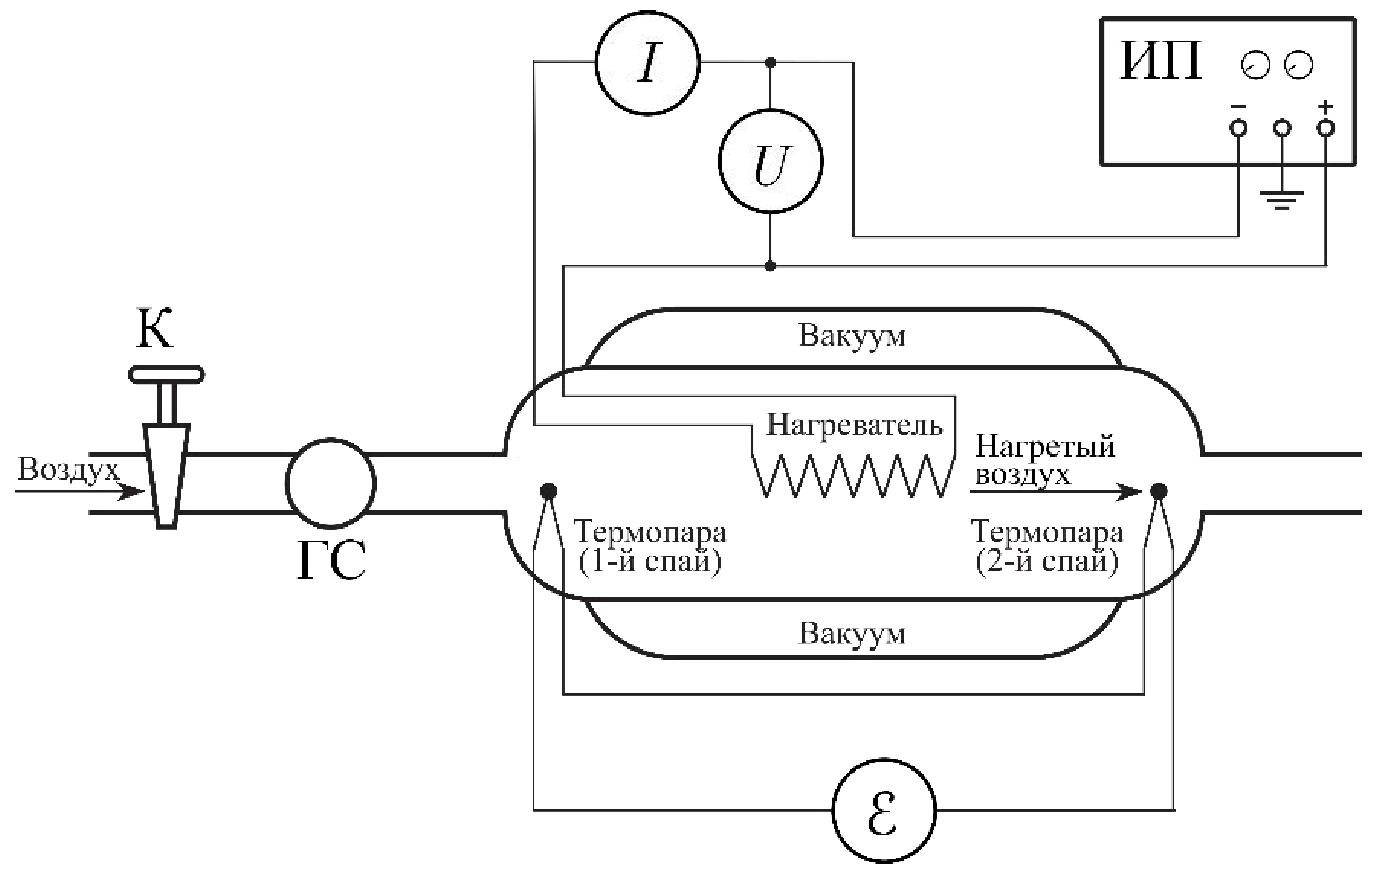
\includegraphics[width=0.8\linewidth]{img/kal.png}
\end{figure}

Воздух, нагнетаемый компрессором, прокачивается через калориметр.
Калориметр представляет собой стеклянную цилиндрическую трубку с двойными стенками,
запаянными с торцов. На внутреннюю поверхность стенок трубки нанесено серебряное покрытие
для минимизации потерь тепла за счет излучения. Воздух из пространства
между стенками калориметра откачан для уменьшения теплопроводности.

Нагреватель расположен в потоке воздуха. Он подключен к источнику питания,
сила тока $I$ и напряжение $U$ которого измеряются мультиметрами. Мощность
нагрева $N=IU$.

Разность температур измеряется по ЭДС $\varepsilon$ на термопаре, спаи которой
находятся в струях входящего и выходящего воздуха. Она пропорциональна
разности температур $\Delta T$: $\varepsilon=\beta\Delta T$.
$\beta=40{,}7\,\frac{\text{мкВ}}{\text{\phantom{}}^\circ\text{С}}$. ЭДС регистрируется микровольтметром.

Обхём воздуха, прошедшего через калориметр измеряется газовым счётчиком.
Для регулировки расхода используется кран. Время прохождения воздуха $\Delta t$
измеряется секундометром. Массовый расход $q$ равен
\[q=\rho_0\frac{\Delta V}{\Delta t}\]
$\rho$~--- плотность воздуха при комнатной температуре.

\[\rho_0=\frac{\mu P_0}{RT_0}\]
$P_0$~--- атмосферное давление, $T_0$~--- комнатная температура, $\mu=29{,}0\,\frac{\text{г}}{\text{моль}}$.

Мощность теплопотерь $N_\text{пот}$ пропорциональна разности температур:
\[N_\text{пот}=\alpha\Delta T\]

Тогда 
\[N=\left(c_pq+\alpha\right)\Delta T\]

В эксперименте следует провести измерение зависимости $\Delta T(N)$ при 
нескольких фиксированных значениях расхода $q$ воздуха.

Важно добиться стационарного состояния. Время установления может достигать 15 минут.
Снятие показаний рекомендуется проводить, когда показания вольтметра, подключенного
к термопаре, не меняются в течение минуты. Охлаждение занимает около 30 минут, поэтому
при измерениях мощность нагрева нужно увеличивать постепенно.
